\SetKw{State}{state}
\SetKw{Send}{send}
\SetKw{Wait}{wait}
\SetKw{Call}{call}
\SetKw{Return}{return}

\SetKwComment{Comment}{//}{}

\SetKwProg{Function}{function}{}{end}

\SetKwBlock{parallelblk}{Do In Parallel}{end}
\SetKwBlock{atomicblk}{atomic}{end}

\SetKwFunction{atomicAdd}{AtomicAdd}
\SetKwFunction{sortps}{sortByLamportEpoch}
\SetKwFunction{executeRetClie}{executeAndSubmitOpReply}
\SetKwFunction{clientSubmit}{Client::SubmitOp}
\SetKwFunction{leaderHandleAccept}{Leader::AcceptRespRecv}
\SetKwFunction{leaderHandleFinalAccept}{Leader::FinalAcceptRespRecv}
\SetKwFunction{clientWait}{Client::SubmitOpReplyRecv}
\SetKwFunction{leaderSubmit}{Leader::SubmitOpRecv}
\SetKwFunction{replicaCoord}{Replica::coordRequestRecv}
\SetKwFunction{shardMain}{Leader::ProcessEpoch}
\SetKwFunction{leaderRecvCR}{Leader::SubmitCRRecv}
\SetKwFunction{CRReply}{Leader::SubmitCRRespRecv}
\SetKwFunction{append}{.append}
\SetKwFunction{find}{.find}
\SetKwFunction{pop}{.pop}
\SetKwFunction{execute}{execute}

\algnewcommand{\IfThenElse}[3]{% \IfThenElse{<if>}{<then>}{<else>}
  \algorithmicif\ #1\ \algorithmicthen\ #2\ \algorithmicelse\ #3}

\algnewcommand{\IfThen}[2]{% \IfThenElse{<if>}{<then>}{<else>}
  \algorithmicif\ #1\ \algorithmicthen\ #2}

\section{\sys{}}
\label{sec:design}
% 1. what are the key features it needs to do. which component of the protocol does that.
% 2. include parts in the motivation that describe why you can't simply do "X". and then in design you can refer to motivation...

\sys{} achieves two goals simultaneously: First, it guarantees \multidispatch{}
linearizability of concurrent requests both within and across clients that span
multiple shards. Second, it achieves lower end-to-end application compared to a
similar (single-dispatch) Linearizable system, while providing the equivalent
ordering guarantees. To do so, \sys{} employs three techniques:

% Design V1: Clients issue multiple ops and send coordination requests to prior ops
% (as in our protocol). Ops are buffered at shard leaders until they are "coordinated."
% The first op in a sequence is trivially coordinated. Once coordinated, an op is
% replicated to a quorum, and then sends a coordination message to next op in sequence.
% Problem: e2e = N * QRT + (N-1) * RTT/2
% Solution: Decouple fault-tolerance from ordering.

First, \sys{} decouples fault-tolerance from ordering by batching each shard's
log into ordering \textit{epochs}. A \sys{} shard replicates and commits
operations as soon as they arrive, but waits to order them as part of an
\textit{epoch}. This allows many concurrent operations to be made fault tolerant
in parallel, deferring ordering to a later sequential step that is amortized
over the operations in an epoch.

Second, \sys{} clients orchestrate coordination between concurrent operations.
This coordination satisfy's \MDL{}'s suffix-complete failure semantics by
ensuring that all of an operation's predecessors are fault tolerant before the
operation itself ordered.


Finally, \sys{} uses Lamport timestamps to guarantee ordering respects
per-client issue order. During the ordering step, a shard assigns a Lamport
timestamp to a committed operation based on the local timestamp and the
timestamp of the operation's dependents.

\sys{}'s full client and shard protocols are specified in
Algorithms~\ref{clientprotocol} and~\ref{shardprotocol} for the client and
server, respectively. We describe each of three techniques in depth below.

% Design V2: Divide log into epochs. Replicate ops in current epoch immediately and allow
% them to send coordination responses. This preserves failure semantics because op is now
% fault-tolerant.
% Feature: improved e2e = 2? * QRT + (N-1) * RTT/2 + E
% Problem: Ops within epoch may not respect issue order across clients.
% Solution: Propagate Lamport timestamps and sort ops in epoch by timestamps.

%% OLD design intro. Some info lost above so make sure it's in the actual sub-sections

%As discussed in Section~\ref{fig:concurrentbatches}, naively allowing
%a client's operations to be ordered separately at multiple shards can lead
%to violations of \MDL{}'s invocation-order guarantees. But many existing
%state-machine replication protocols, including Raft, couple fault-tolerance
%and ordering. Thus, it would seem that to guarantee both per-client issue order
%and suffix-complete failure semantics, each operation must wait to replicate
%until after its predecessor finishes replicating (and thus being ordered).
%Unfortunately, the end-to-end latency of an application issuing $N$ operations
%to such a system would be approximately $N$ times one quorum round-trip plus
%one inter-shard message. This is worse than linearizable Raft, which just requires
%one quorum round-trip per operation.
%
%To offer lower end-to-end application latency, \sys{} thus decouples
%fault-tolerance from ordering by dividing each shard's log into \textit{epochs}.
%An operation is first replicated as part of a \textit{pending operation set},
%after which it can notify its successor. This replication can proceed in
%parallel for all operations in a client's sequence. At the end of each epoch,
%the operations in the pending operation set are ordered by placing them into
%the shard's log, requiring a second quorum round trip.
%
%% Design V3: Our full protocol.
%
%Finally, to ensure per-client issue order is respected both within and across
%shard epochs, \sys{} assigns each operation a Lamport timestamp and sorts each
%epoch's operations by their timestamps. Upon arrival at a shard, an operation
%is assigned an initial, tentative timestamp based on the maximum of the timestamps of
%all operations that have been replicated and coordinated previously at the shard.
%Operations then propagate these timestamps to the successors in their coordination
%messages, and successors update their timestamps to always be greater than their
%predecessors.

% Jeff: I think this is mostly covered (or will be) in the previous two sections.
% Existing protocols that provide \sdl assume clients abide by the restriction to single-dispatch requests, having at most one outstanding request at a time. This assumption comes from the definition of linearizability, which requires individual clients to behave sequentially. These protocols, such as Paxos, Raft, Viewstamped Replication, Zab, do not provide any guarantees on the order that concurrent requests issued from a single client take effect. Our definition of \md specifies that concurrent requests issued from a single client take effect in invocation order. 

\begin{figure}[!htb]
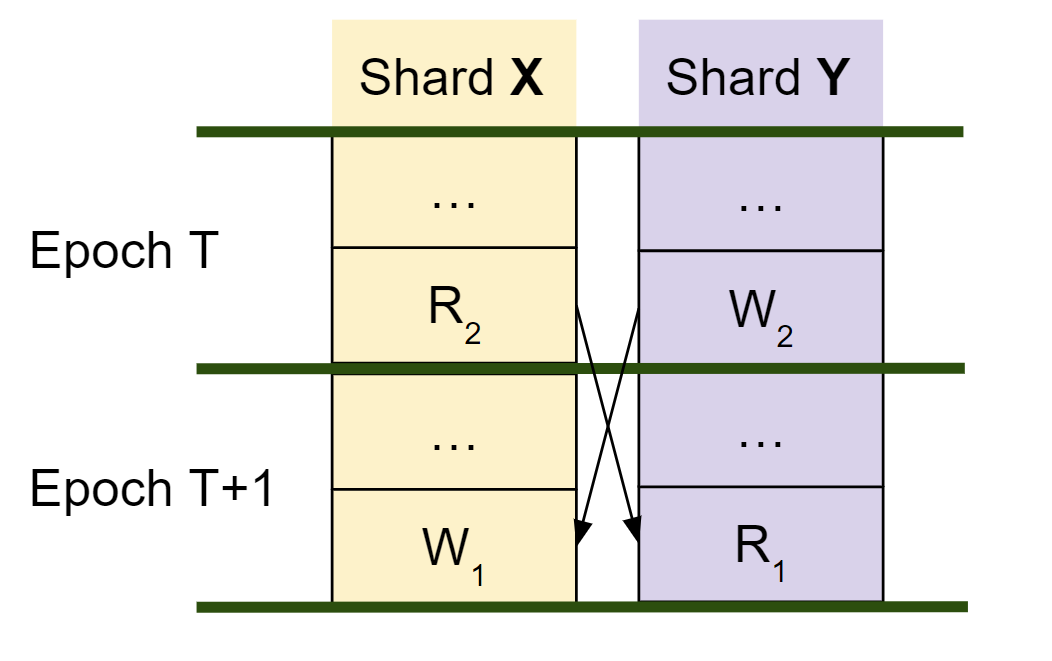
\includegraphics[scale=.3]{figs/sorted_batching_wrong.png}
\caption{Example execution of sorted batching without coordination requirement. This execution leads to an incorrect execution that contains a cycle and is not \mdl. The execution is the same execution as that of figure \ref{fig:concurrentbatches}, but now the second request issued by each client arrives in an earlier epoch. Even if sorted in their respective epochs, they are not ordered across epochs without coordination.}
\label{fig:sortedbatchingwrong}
\end{figure}

% Since all requests can not be known a priori, we make use of epochs at each shard, and guarantee sorted execution order within each epoch, as well as a safe ordering across epochs. With this approach, we can prune request interleavings that might lead to cycles upfront, rather than running cycle detection and subsequently failing execution. While this unnecessarily prevents some subset of safe interleavings, the latter scales poorly for very large cycles.

\subsection{Decoupling Fault-Tolerance \& Ordering}

Operations in a multi-shard system can fail independently, e.g., during leader
failure at one shard. Naively ordering a client's concurrent operations
independently at multiple shards, as many existing state-machine replication
protocols do, would violation \MDL{}'s invocation-order guarantee. On the other
hand, blocking operations on one shard on the completion of previously-invoked
operations on other shards in these systems would be impractically slow. The
problem is that existing state-machine replication protocols couple
fault-tolerance and ordering---e.g.\ leaders replicate both the operation itself
and its order in the log simultaneously. In order to guarantee suffix-complete
failure semantics, operations cannot be replicated until their predecessors have
also been replicated.

%The end-to-end latency of an application issuing $N$ operations to
%such a system would be approximately $N$ times one quorum round-trip plus one
%inter-shard message. This is worse than linearizable Raft, which just requires
%one quorum round-trip per operation.

A key insight of \sys{} is to decouple fault-tolerance from ordering, allowing
replication of concurrent operations to proceed in parallel on different shards,
separate from ordering. While in existing state-machine replication protocols
operations are either committed or uncommitted, operations in \sys{} can be in
one five states: \textit{pending}, \textit{committed} but not
\textit{coordinated}, \textit{coordinated} but not \textit{committed},
\textit{committed} and \textit{coordinated}, and \textit{ordered}.

When an operation arrives at a shard leader, it is \textit{pending}. Once the
shard has replicated the operation to a quarum of replicas, the operation
becomes \textit{committed}, and the shard can respond to the client. A
\textit{committed} is guaranteed not to fail---i.e.\ it is guaranteed to
eventually be ordered, even under, e.g., leader changes. Operations are
considered \textit{coordinated} once all of their predecessors (operations
invoked earlier by the same client) are both committed and coordinated.
Operations with no predecessors are immediately coordinated. Once an operation
is both committed \emph{and} coordinated, it can added to the ordered log.  An
operation that has been included in the ordered log at both a leader and a
quorum of replicas is considered \textit{ordered}. Leaders and replicas execute
ordered requests in the same fashion as Raft~\cite{ongaro2014raft}, and leaders
respond to clients after executing an operation.

Note that committing an operation for fault-tolerance, and coordinating it to
ensure invocation order with predecessors happen asynchronously. This allows
concurrent operations to be committed in parallel, and coordination to make
progress concurrently with commitment, deferring ordering until both have
completed.

However, as a result, each operation requires two rounds between a shard leader
and a quorum of its replicas. When the operation arrives at the shard leader, it
is replicated first for fault-tolerance and placed into a pending operation set.
Once the operation is \textit{coordinated}, the leader must again replicate its
\emph{order}. \sys{} amortizes replication of the order by dividing the
execution of operations at each shard into a series of \textit{epochs}. At the
end of each epoch, operations from the pending set that have been coordinated
are sorted (Section~\ref{sec:design:timestamps}) and their order replicated to a
quarum in batch.

Operation in the pending set may fail to be included in the current epoch for
one of two reasons: (1) they may time out while waiting to receive a
coordination response from their predecessor, which we implement by bounding the
number of epochs during which it can exist in the pending operation set, or (2)
they may receive an explicit FAIL response for its coordination response. The
latter can happen if, for instance, a leader failure occurred at one of the
predecessors' shards.

\al{I don't understand the FAIL thing}

\subsubsection{Operation vs. End-To-End Latency}

Although decoupling fault-tolerance and ordering increases each operation's latency by introducing a
second round of messages between a leader and its replicas, it still improves end-to-end application
latency of applications that issue more than a few operations. This is because shards can replicate
operations from the same client in parallel. As described in the section below, using Lamport timestamps,
shards can safely order and execute operations in parallel, too. Thus, only the cross-shard coordination
messages are sent sequentially for a client's sequence of operations.

As a result, a client's end-to-end application latency when using \sys{} scales by a factor
of the one-way cross-shard latency as the number of operations increases. In contrast,
the latency of applications using a \singledispatch{} system scales by a factor of the
quorum round-trip latency. Our evaluation in Section~\ref{sec:eval} bears out this claim.

\subsection{Client-Driven Coordination}

\sys{} shards coordinate with each other to ensure that operations are applied
according to the client's invocation order. But how do shards know which
operations are dependent on each other? One option would be for the client to
propagate dependencies along with each operation---each operation would include
the predeceeding concurrent requests that were invoked before it. However, this
would require an additional message from the shard responsible for an operation
and the shard of its predecessor to request coordination.

Instead, \sys{} introduces client-driven \textit{coordination requests (CR)},
that parallelize coordination requests with the operations themselves.  When a
client submits an operation to a shard, it also submits a CR, in parallel, to
the shard of its predecessor operation with the identity of the shard of its
successor.  In particular, for some operation issued by client $C$ with sequence
number $s$, a predecessor operation is defined as the concurrent operation that
client $C$ issued with sequence number $s-1$. If client $C$ does not have any
other outstanding operations, then the operation's predecessor is \texttt{null}.

Upon receiving a coordination request, a shard first waits until the operation
is committed and coordinated and then sends a \textit{coordination response} to
the shard leader of its successor. This inductively guarantees all of an
operation's predecessors will eventually succeed. An operation is considered
\textit{coordinated} if the shard has received a \textit{coordination response}
from the shard leader of the operation's predecessor.  (Operations without a
predecessor are vacuously coordinated.)

\subsection{Lamport Timestamps For Issue Order}\label{sec:design:timestamps}

To ensure operations end up in a valid \MDL{} order, \sys{} assigns each operation a Lamport timestamp.
Operations are then sorted by their timestamp values (using arrival time at the shard to break ties)
at the end of an epoch.

Operations are assigned to maintain three invariants: (1) Each operation's timestamp must
be strictly greater than the timestamps of any operations that were previously replicated and coordinated
at the same shard; (2) an operation's timestamp is strictly greater than its predecessor's; and (3)
the timestamp of the first operation in each epoch is strictly greater than that of the last operation
in the previous epoch. 

To do so, each shard shard maintains a \texttt{next\_ts} integer, initially zero, that is advanced whenever
an operation is replicated and coordinated and at the end of each epoch. Upon arriving at a shard, an operation
sets its tentative timestamp as the current value of \texttt{next\_ts}. An operation's timestamp is then
finalized when it becomes coordinated and committed. Predecessors include their timestamps in their coordination
responses. Successor operations then ensure that their timestamp is strictly greater than that
of their predecessor. At the end of an epoch \texttt{next\_ts} is advanced to be strictly greater than the last
operation in the epoch.

TODO: Add intuition about why these invariants are needed.

% \md can only guarantee a safe total ordering across epochs of shards if it executes \textit{ordered} requests. Figure ~\ref{fig:sortedbatchingwrong} shows an execution that does not abide by this constraint, and only sorts committed (but not coordinated) requests within epochs. A cycle arises among all the requests across epoch boundaries, thus the execution does not have a total order and is not multi-dispatch linearizeable. A SUCCESS response for a given request's CR message, which coordinates it, serves as a promise that all predecessors have been sorted at the same or earlier epochs on their respective shards, which provides a total order across epochs of different shards.

% To to get invocation order, there are multiple mechanisms at play
% 1. sequence numbers
% 2. CR requests that are issued by clients
%       -these only get sent to the immediate predecessor (talk about inductive guarantees)
%       -these only get acked if all the other predecessors have been acked too, guaranteeing they are sorted as well. you can only be in an epoch equivalent to or greater than the epochs of your predecessors (not absolute values)

% Ensure that epcoh increase monotonically
% ensure that each epoch is executed in sorted order
% ensure that across epoch boundaries nothing fishy happens, guaranteed via CR acks
% ensure we have the extra round trip at the end to "order" commands (this is for failure too??)

% \subsection{Batching}
% \md makes use of batching to increase throughput and amortize the \textit{ordering} inter-replica round trip across multiple requests in an epoch. Multi-dispatch linearizeable back-end systems expect to experience more load than their single-dispatch linearizeable counterparts, since individual clients can issue many more requests in the former. For example, for $k$ shards, if clients submit on average 10 requests at a time, the logs at shards of \md backends will be about $10/k$ times longer than the logs of \sd shards. Thus batching is a nice way to handle processing of congested shard logs. Moreover, our coordination mechanism is independent across requests from different clients, thus we do not introduce any head-of-line blocking. For requests that arrive later but become coordinated sooner, those can be executed immediately without waiting on the coordination of requests from separate clients.
% Comment that we expect a more congested log at each shard since now there will be fanout from individual clients
% batching is a nice fit since it can exploit this high load
% moreover, ordering a request does not depend on previously arrived requests from independent clients to be ordered, hwich is a nice design that allows each client to see issue order scale with just their behavior, not other clients'.

\begin{figure}
\begin{tikzpicture}
[box/.style={draw=none, thick, font=\small, text centered, minimum height=1.2cm, minimum width=1.0cm}]
\newcommand\w{3}
\newcommand\h{5}

\node (clientbox) [box, yshift=6.5cm] {$C$};

\node (leaderbox) [box, yshift=6.5cm, xshift=\w cm] {$L_1$};

\node (replicabox) [box, yshift=6.5cm, xshift=2*\w cm] {$R$};
% C
\draw [stealth-](0,0) -- (0,\h+1);
% L1
\draw [stealth-](\w,0) -- (\w,\h+1);
% R1
\draw [stealth-](2*\w,0) -- (2*\w,\h+1);

% Left T{
\draw [decorate,
    decoration = {brace}] (\w-0.05,-0.15) --  (0,-0.15);
\node [box, yshift=-0.5cm, xshift=0.5*\w cm] {$T$};

% Right T{
\draw [decorate,
    decoration = {brace}] (2*\w,-0.15) --  (\w+0.05,-0.15);
\node [box, yshift=-0.5cm, xshift=1.5*\w cm] {$T$};


% Req1
\node [box, yshift=4.5cm, xshift=6.5cm] {$Req_1$};
% Top 4*T {
\draw [decorate,
    decoration = {brace}] (-0.15,4) --  (-0.15,5);
\node [box, yshift=4.5cm, xshift=-0.75 cm] {$4*T$};

% Req2
\node [box, yshift=3.25cm, xshift=6.5cm] {$Req_2$};
% Middle 4*T {
\draw [decorate,
    decoration = {brace}] (-0.15,2.75) --  (-0.15,3.75);
\node [box, yshift=3.25cm, xshift=-0.75 cm] {$4*T$};

% ReqN
\node [box, yshift=1.25cm, xshift=6.5cm] {$Req_N$};
% Bottom 4*T {
\draw [decorate,
    decoration = {brace}] (-0.15,0.75) --  (-0.15,1.75);
\node [box, yshift=1.25cm, xshift=-0.75 cm] {$4*T$};

% First request message < 4 Ts
\draw [-stealth](0,\h) -- (\w,0.95*\h);
\draw [-stealth](\w,0.95*\h) -- (2*\w,0.9*\h);
\draw [-stealth](2*\w,0.9*\h) -- (\w,0.85*\h);
\draw [-stealth](\w,0.85*\h) -- (0,0.8*\h);

% Second request messages < 8 Ts
\draw [-stealth](0,0.75*\h) -- (\w,0.7*\h);
\draw [-stealth](\w,0.7*\h) -- (2*\w,0.65*\h);
\draw [-stealth](2*\w,0.65*\h) -- (\w,0.6*\h);
\draw [-stealth](\w,0.6*\h) -- (0,0.55*\h);

% ellipses ...
\draw (0.2*\w,0.45*\h) node[auto=false]{\ldots};

% Last request message < 4*N Ts
\draw [-stealth](0,0.35*\h) -- (\w,0.3*\h);
\draw [-stealth](\w,0.3*\h) --  (2*\w,0.25*\h);
\draw [-stealth](2*\w,0.25*\h) -- (\w,0.2*\h);
\draw [-stealth](\w,0.2*\h) -- (0,0.15*\h);
\end{tikzpicture}
\caption{Performance for SDL. Since clients must issue requests sequentially, we expect N requests issued to take around $4*T*N$ units of time, where $T$ is the latency between servers. In our case we assume this latency is equivalent between clients and leaders, as well as leaders and replicas. We only display a single shard case since the latency should be equivalent for multiple shards.}
\label{fig:sdlperf}
\end{figure}
%%%%%%%%%%%%%%%%%%%%%%%%%%%%%%%%%%%%%%%%%%%%%%%%%%%%%%
\begin{figure}
\begin{tikzpicture}
[box/.style={draw=none, thick, font=\small, text centered, minimum height=1.2cm, minimum width=1.0cm}]
\newcommand\w{0.8}
\newcommand\h{4.5}
\tikzset{snake it/.style={decorate, decoration=snake}}

\node (clientbox) [box, yshift=6cm] {$C$};

\node (leaderbox) [box, yshift=6cm, xshift=\w cm] {$L_1$};

\node (replicabox) [box, yshift=6cm, xshift=2*\w cm] {$R_1$};

\node (leaderbox) [box, yshift=6cm, xshift=3*\w cm] {$L_2$};

\node (replicabox) [box, yshift=6cm, xshift=4*\w cm] {$R_2$};

\node (leaderbox) [box, yshift=6cm, xshift=7*\w cm] {$L_N$};

\node (replicabox) [box, yshift=6cm, xshift=8*\w cm] {$R_N$};

% Client
\draw [stealth-](0,0) -- (0,\h+1);

% L1, R1
\draw [stealth-](\w,0) -- (\w,\h+1);
\draw [stealth-](2*\w,0) -- (2*\w,\h+1);

%L2, R2
\draw [stealth-](3*\w,0) -- (3*\w,\h+1);
\draw [stealth-](4*\w,0) -- (4*\w,\h+1);

%LN, RN
\draw [stealth-](7*\w,0) -- (7*\w,\h+1);
\draw [stealth-](8*\w,0) -- (8*\w,\h+1);

% Left T{
\draw [decorate,
    decoration = {brace}] (\w-0.05,-0.15) --  (0,-0.15);
\node [box, yshift=-0.5cm, xshift=0.5*\w cm] {$T$};

% Right T{
\draw [decorate,
    decoration = {brace}] (2*\w,-0.15) --  (\w+0.05,-0.15);
\node [box, yshift=-0.5cm, xshift=1.5*\w cm] {$T$};

% L2--LN T{
\draw [decorate,
    decoration = {brace}] (7.05*\w-0.05,-0.15) --  (3*\w,-0.15);
\node [box, yshift=-0.5cm, xshift=5*\w cm] {$T$};

% N request messages
\draw [-stealth](0,\h+0.6) -- node[midway,fill=white]{\footnotesize $R_1$}(\w,\h+0.2);
\draw [-stealth](0,\h+0.6) to[out=10, in=-200] node[midway,fill=white]{\footnotesize $R_2$} (3*\w,\h+0.2);
\draw [-stealth](0,\h+0.6) to[out=30, in=-200] node[midway,fill=white]{\footnotesize $R_N$} (7*\w,\h+0.2);

\draw [-stealth](0,\h+0.6) to[out=19, in=-190] (2.3*\w,\h+0.9);

% N paxos round trips
\draw [-stealth](\w,\h+0.2) -- (2*\w,\h-0.2);
\draw [-stealth](2*\w,\h-0.2) -- (\w,\h-0.6);

\draw [-stealth](3*\w,\h+0.2) -- (4*\w,\h-0.2);
\draw [-stealth](4*\w,\h-0.2) -- (3*\w,\h-0.6);

\draw [-stealth](7*\w,\h+0.2) -- (8*\w,\h-0.2);
\draw [-stealth](8*\w,\h-0.2) -- (7*\w,\h-0.6);

% First CR resp and client response
\draw[-stealth, dashed] (\w,\h-0.6) -- node[midway,fill=white]{\tiny $Coord_2$}(3*\w,\h-1);
\draw [-stealth](\w,\h-0.6) -- (0,\h-1);

% second CR resp and client response
\draw[-stealth, dashed] (3*\w,\h-1) -- node[midway,fill=white]{\tiny $Coord_2$}(5*\w,\h-1.4);
\draw [-stealth](3*\w,\h-1) -- (0,\h-1.4);

% Nth CR resp and client response
\draw[-stealth, dashed] (5*\w,\h-2.25) -- node[midway,fill=white]{\tiny $Coord_N$}(7*\w,\h-2.75);
\draw [-stealth](7*\w,\h-3.55) -- (0,\h-3.95);

% Ellipses
\draw (5*\w,\h-1.85) node[auto=false]{\ldots};
\draw (2.35*\w,\h+0.8) node[auto=false]{\ldots};
%Final Paxos round trip
\draw [-stealth](7*\w,\h-2.75) -- (8*\w,\h-3.15);
\draw [-stealth](8*\w,\h-3.15) -- (7*\w,\h-3.55);

% Brackets
\draw [decorate,
    decoration = {brace}] (-0.15,\h-0.57) --  (-0.15,\h+0.6);
\node [box, yshift=\h cm, xshift=-0.7 cm] {$3*T$};

\draw [decorate,
    decoration = {brace}] (-0.15,\h-2.75) --  (-0.15,\h-0.6);
\node [box, yshift=0.63*\h cm, xshift=-1.15 cm] {$(N-1)*T$};

\draw [decorate,
    decoration = {brace}] (-0.15,\h-3.95) --  (-0.15,\h-2.8);
\node [box, yshift=0.2*\h cm, xshift=-0.7 cm] {$3*T$};

% Horizontal lines
\draw[dashed] (0,\h+0.2) -- (8*\w,\h+0.2);
\draw[dashed] (0,\h-0.6) -- (8*\w,\h-0.6);
\draw[dashed] (0,\h-2.75) -- (8*\w,\h-2.75);


\end{tikzpicture}
\caption{Performance for MDL. Ommitted: Client issued coordination requests and final paxos ordering round trip for all requests except $R_N$ (shown). Since clients can issue multiple outstanding requests, we expect N requests issued to take around $6T + (N-1)*T$ units of time, where $T$ is the latency between servers and $N$ is the number of unique shards across all outstanding requests. In our case we assume this latency is equivalent between clients and leaders, leaders and replicas, as well as leaders to leaders.}
\label{fig:mdlperf}
\end{figure}

\subsection{Correctness}
We give a brief sketch of correctness for \protocol, showing why it guarantees \mdl. A more detailed discussion on leader failures follows in section ~\ref{subsec:leaderfailures}. We provide a full proof of correctness in our technical report ~\ref{}.

To guarantee \mdl, our protocol must provide a total order of operations that (1) respects per-client invocation order, (2) respects real time, and (3) respects our failure semantics. 

Our coordination request mechanism provides \md's failure semantics and also offers a vehicle to pass along lamport timestamps that can guarantee a safe linearization. Because requests coordinate their successors \textit{after} they themselves are coordinated and committed, the lamport timestamps they send include all causal relationships about requests ordered ahead of them in their log as well as requests invoked earlier by the same client. 
% Since shard leaders update their global timestamps immediately when requests are committed, coordinated, and added to the ordered log, the timestamps sent to successors also carry execution causal relationships within shards. 
Inductively, this ensures that all concurrent successors from the same client at possibly different shards carry these log and invocation orderings. Our coordination mechanism is also strong enough to provide real time guarantees.

Lastly, coordination requests provide our failure semantics by forwarding information about success and failures. If a request fails, all successors will either be notified of this failure and thus fail themselves and all successors, or, if not notified after a timeout period, they will pessimistically assume a failure and proceed to also fail themselves and their successors. This ensures a suffix closed set of failures, preceeded by a prefix closed set of successes.

\subsection{Leader Failure}
\label{subsec:leaderfailures}
To begin, we employ a similar voting mechanism as Raft for selecting the leader from the candidate from the highest term that has the most up-to-date log, where in this case the log is the ordered log of requests that were sorted and executed in prior epochs. This ensures that all committed and executed (and possibly client-externalized) requests are in all future leader logs. Next we describe how buffered requests are safely carried across successive terms with different leaders.

During operation of \protocol, requests can exist in multiple intermediate states. Specifically, a failure could occur after a request has (1) arrived in the buffered map, (2) been committed, (3) received a coordination response from its predecessor, (4) been added to the execution log (5) coordinated its successor request, (6) been committed in the execution log in this term, (7) been executed, or (8) responded to the client. 

The interesting case to look at is a failure right after point (5). Any request $r$ that has already coordinated a successor request \textit{must} (A) be in the future logs of all leaders, to provide failure semantics, and (B) be placed in the correct order in the log post-failure, to guarantee invocation ordering. These guarantees are less important for requests that have not coordinated a successor since those requests have no impact on successors that might externalize this state, and clients can simply reissue these requests if they fail/are lost. 

To guarantee (A), after an election completes, any new leader must ask for the buffered logs of at least a quorum of replicas to ensure it has every request that might have successfully coordinated a successor requests. We do not replicate the coordination bit on non-leader nodes, since this would diminish our opportunity to parallelize coordinating an entry and making it fault tolerant. By extension, knowledge of which requests have coordinated their successors only exists at the leader, this information is also not replicated. Because of this, there is no way for a new leader to know which buffered entries are coordinated themselves or have coordinated successor requests, so it performs this log diff. This technique is similar to View-Stamped Replication's ~\ref{} \texttt{DoViewChange} messages sent from replicas to leaders during a view change. 

Crucially, if this step is omitted, a leader might be elected that is missing an entry that coordinated a successor request. For example, consider a network partition which creates two subclusters, each of which contains a node operating as a leader (one in a later term than the other). The subcluster that contains a quorum could receive a request and in the future coordinate its successor at another shard after it itself has been committed and coordinated. Consider when the leader of this subcluster fails to deliver the commit messages to replicas to order this entry at this log index, and immediately afterwards the partition is removed. At this point, no replica that might become a leader is aware of the fact this entry has coordinated its successor, or even that it has moved from the buffered map and to the ordered log. There is no available information among the replicas to reconstruct this information, so we must pessimistically assume all buffered entries at a quorum of nodes have coordinated their successors and include them in the buffered log of the newly elected leader.

To provide (B), at the beginning of each new term, a newly elected leader must immediately process all buffered entries and place them in the ordered log before accepting any future client requests (or fail them if their predecessors failed). This is an expensive task during which the new leader must reissue each buffered request's coordination message (that the client sent initially) to the predecessor shard and wait for a response. In parallel, the new leader must also replicate each buffered request at a new quorum of nodes to ensure the entry exists on a quorum of replicas across multiple leader failures (the buffered log is not persisted). 

As the new buffered entries at the new leader become committed and coordinated, we do not immediately add them to the ordered log. Moreover, we do not update the global shard timestamp between each commit/coordination event. Finally, once the last buffered entry is committed and coordinated, we enter all entries in sorted timestamp order to the ordered log (or fail them if their predecessor failed). Without this expensive buffer flushing, it is possible that a new request $r'$ might arrive and become committed and coordinated before a buffered entry $r$ that was committed and coordinated at the previous leader is committed and coordinated with the current leader. Linearizability could be violated if $r'$ must be ordered in the log after $r$ but is placed in the ordered log before $r$. The lamport timestamps guarantee a safe total ordering that respect any causal relationships. While we might reorder operations that are not causally related, this is safe and does not violate \mdl. 

Finally, we mention that coordination requests might also be lost in the network or across leader failures. To solve this, each request has a fixed amount of total epochs for which it can remain uncoordinated. After a leader sees that a request is "stale", it will fail the request as well as any pending coordination requests from successors of that request, beginning the suffix closed failure set. This solution also handles the garbage collection of the buffered log.

%%%%%%%%%%%%%%%%%%%%%%%%%%%%%%%%%
%%%%%%%%% Client %%%%%%%%%%%%%%%%
%%%%%%%%%%%%%%%%%%%%%%%%%%%%%%%%%
\begin{algorithm}
    \State $PID \gets$ unique client ID\\
    \State $\mathcal{L} \gets \{...\}$ \algorithmiccomment{Shard Leaders}\\
    \State $i \gets 0$ \algorithmiccomment{Sequence No Per Shard}\\
    \State $prevReq \gets NULL$\\
    %\State $m$ \algorithmiccomment{mutex}\\
    \Function{\clientSubmit{Op, K, V}}{
        $seqno := i$\\
        $i\mathrel{+}=1$\\
        $Req := (Op, K, V, PID, seqno)$\\
        %$m.lock()$ \algorithmiccomment{Critical section begins}\\
        $prq := prevReq$\\
        $prevReq \gets Req$\\
        %$m.unlock()$ \algorithmiccomment{Critical section begins}\\
        \IfThen{$prevReq \neq NULL$}{\Send $SubmitCR(prq, Req)$ to $L_{K-1} \in \mathcal{L}$}\\
        \Send $SubmitOp(Req)$ to $L_K \in \mathcal{L}$\\        
    }

    \Function{\clientWait{Req}}{
        \Wait receive $SubmitOpReply(V)$ from $L_K \in \mathcal{L}$\\
        %$m.lock()$\\
        $\IfThen{prevReq = Req}{prevReq \gets NULL}$\\
        %$m.unlock()$\\
        \Return $V$\\
    }
    \caption{MD-Lin Client}
    \label{clientprotocol}
\end{algorithm}
%%%%%%%%%%%%%%%%%%%%%%%%%%%%%%%%%
%%%%% Shard Leader %%%%%%%%%%%%%%
%%%%%%%%%%%%%%%%%%%%%%%%%%%%%%%%%
% \begin{algorithm}
%     \State $ShardTS \gets 0$\\
%     \State $Timer \gets T$\\
%     \State $accepting \gets True$\\
%     \State $bufferedMap \gets []$\\
%     \State $orderedLog \gets []$\\
%     \State $ClientSeqnoMap \gets [][]$\\
%     \Function{\shardMain{}}{
%         \Wait until $Timer = 0$\\
%         $accepting \gets False$\\
%         $batch := []$\\
%         \For{$entry \in bufferedMap$\\}{
%             $entry.epochsSeen\mathrel{+}=1$\\
%             \If{$entry.committed \land entry.coordinated$\\}{
%                 %$entry.epoch \gets ShardTS$\\
%                 $batch\append{entry}$\\
%                 $ShardTS = Math.max(ShardTS, entry.epoch)$\\
%                 $bufferedMap\pop(entry)$\\
%             }
%             \ElseIf{$entry.epochsSeen > MAX\_EPOCHS$}{
%                 $bufferedMap\pop(entry)$\\
%                 $SubmitCRResp(entry, False)$ to $L_{K+1} \in \mathcal{L}$\\
%             }
%         }
%         \sortps{batch}\\
%         $orderedLog\append{batch}$\\
%         $ShardTS \mathrel{+}=1$\\
%         \Send $FinalAppendEntries(batch)$ to all $r \in \mathcal{R}$\\
%         %\Wait receive $AppendEntriesSuccess$ from all $r \in Q \in \mathcal{R}$\\
%         %$bufferedMap\popO{}$\\
%         $\executeRetClie{batch}$\\
%         %$\atomicAdd(ShardTS, 1)$\\
%         $accepting \gets True$\\
%         $Timer \gets T$\\
%     }
%     \caption{MD-Lin Shard Leader Epoch Handling}
%     \label{shardprotocolmain}
% \end{algorithm}
\begin{algorithm}
    \Function{\leaderSubmit{Op, K, V, P, s}}{
        \If{$ClientSeqnoMap[P] \neq s$}{
            $buffer_{P}(\{Op, K, V, P, s\})$\\
            \algorithmiccomment{Buffer per-client out of order requests}\\
            \Return\\
        }
        \Wait until $accepting = True$\\
        \algorithmiccomment{Issue this op}\\
        $bufferedMap\append{(Op, K, V, P, s, 0)}$\\
        $ClientSeqnoMap[P]\mathrel{+}=1$\\
        \Send $Accept(Op, K, V, P, s)$ to all $r \in \mathcal{R}$\\
        \For{$(Op, K, V, P, s) \in buffer_{P}$}{
        \algorithmiccomment{Issue OoO buffered ops that are now ready}\\
            \If{$ClientSeqnoMap[P] = s$}{
                $bufferedMap\append{(Op, K, V, P, s, 0)}$\\
                $ClientSeqnoMap[P]\mathrel{+}=1$\\
                \Send $Accept(Op, K, V, P, s)$ to all $r \in \mathcal{R}$\\
            }
        }
    }
    \Function{\leaderHandleAccept{req}}{
        $req.acks\mathrel{+}=1$\\
        \If{$req.acks \ge |Q|$} {
             $req.committed \gets True$\\
        }
        \If{$req.committed \land req.coordinated$}{
            $req.ts := \max(req.ts+1, ShardTS)$\\
            $ShardTS := \max(req.ts, ShardTS)+1$\\
            $SubmitCRResp(req.succrq, True, req.ts)$ to $L_{K+1} \in \mathcal{L}$\\
            $bufferedMap\pop(req)$\\
            $orderedLog\append{req}$\\
            \Send $FinalAccept(req)$ to all $r \in \mathcal{R}$\\            
        }
    }
    \Function{\leaderHandleFinalAccept{req}}{
        $req.facks\mathrel{+}=1$\\
        \If{$req.facks \ge |Q|$}{
            $v := \execute{req}$\\
            $SubmitOpReply(req, v)$ to $client$\\
            \Send $Commit(req)$ to all $r \in \mathcal{R}$\\
        }
    }   
    \caption{MD-Lin Shard Leader Communication}
    \label{shardprotocolmessages}
\end{algorithm}
\begin{algorithm}
    \Function{\leaderRecvCR{rq, succrq}}{
    \algorithmiccomment{Received CR from client of succrq}\\
        $rq.succrq := succrq$\\
        \If{$entry := orderedLog\find{rq} \neq NULL$}{
            $SubmitCRResp(succrq, True, entry.ts)$ to $L_{K+1} \in \mathcal{L}$\\
            \Return\\
        }
        \Wait $entry := bufferedMap\find{rq} \neq NULL$\\
        \Wait $(entry.committed \land entry.coordinated) \lor bufferedMap\find{rq} = NULL$\\
        \If{$entry.committed \land entry.coordinated$}{
            $SubmitCRResp(succrq, True, entry.ts)$ to $L_{K+1} \in \mathcal{L}$\\
        }
        \Else{
            $SubmitCRResp(succrq, False, -1)$ to $L_{K+1} \in \mathcal{L}$\\
        }        
    }
    \Function{\CRReply{req, v, ts}}{
        
        \If{$v = True$}{
            % \Wait $entry := bufferedMap\find{rq} \neq NULL$\\
            $req.coordinated \gets True$\\
            $req.ts = ts$\\
            \If{$req.committed \land req.coordinated$}{
                $req.ts := \max(req.ts+1, ShardTS)$\\
                $ShardTS := \max(req.ts, ShardTS)+1$\\
                $SubmitCRResp(req.succrq, True, req.ts)$ to $L_{K+1} \in \mathcal{L}$\\
                $bufferedMap\pop(req)$\\
                $orderedLog\append{req}$\\
                \Send $FinalAccept(req)$ to all $r \in \mathcal{R}$\\            
            }
        }
        \Else{
            $bufferedMap\pop(rq)$\\
            $SubmitCRResp(rq.succrq, False, -1)$ to $L_{K+1} \in \mathcal{L}$\\
        }
    
    }
    \caption{MD-Lin Shard Leader Coordination}
    \label{shardprotocolcoord}
\end{algorithm}

